\documentclass{article}
\usepackage[utf8]{inputenc}
\usepackage[english]{babel}



% Keywords command
\providecommand{\keywords}[1]
{
  \small	
  \textbf{\textit{Keywords---}} 
}

\title{Como fazer consultas a bancos de dados relacionais sem conhecer SQL?}
\author{Henrique Bueno Rodrigues}
\date{November 2018}

\usepackage{natbib}
\usepackage{graphicx}

\begin{document}

\maketitle
\begin{abstract}
Apesar do advento de tecnologias de bancos de dados não convencionais, por exemplo, NoSQL, um grande volume de dados permanece armazenado em repositórios relacionais. Além disso, a necessidade de consumir dados de uma forma mais simples e amigável é exigida por usuários que desejam explorar suas informações com maior liberdade. A recente primavera das técnicas de Inteligência Artificial, com destaque para aquelas relacionadas à Processamento de Linguagem Natural, renovou as esperanças de obtenção de novos avanços nas interfaces de acesso a bancos de dados. Este trabalho apresenta um levantamento dos diferentes modelos de sistemas "Natural Language Interface to Database" (NLIDB), que são sistemas de consulta a bancos de dados relacionais à partir de pesquisas escritas em linguagem natural.
\end{abstract}

\section{Introdução}

Linguagem. Essa é uma das principais formas pela qual humanos expressam suas ideias, se comunicam e se inspiram \citep{harari2014sapiens}.\\

Desde o surgimento dos computadores há o desejo de transferir a capacidade de comunicação às máquinas. 
%Isso fica evidente através de computadores famosos do cinema, por exemplo, HAL-9000 \citep{hal9000}.\\

VER MOTIVAÇÕES DE OUTROS TRABALHOS\\

Um exemplo de tarefa que sempre se desejou transferir às máquinas é a capacidade de responder perguntas. Dentro da ciência da computação, a linha de estudo que investiga sistemas capazes de responder perguntas escritas em linguagem natural é chamada Question Answering (QA) \citep{hirschman2001natural}.\\

Problemas do tipo QA podem ser classificados de acordo com suas características, por exemplo: domínio das perguntas, tipo das perguntas e tipo das fontes de dados \citep{mishra2016survey, speech}.\\

O domínio das perguntas pode ser aberto (geral) ou fechado (restrito). No caso do domínio aberto, as perguntas não são específicas de um nicho de conceitos ou entidades, elas são perguntas gerais. Por outro lado, no caso do domínio fechado, as perguntas são de um escopo determinado e restrito.\\

Os tipos de perguntas podem ser factóide, lista, hipotética, causal e confirmação. O tipo factóide representa perguntas sobre fatos, por exemplo, "Quem é o presidente do Brasil?". O tipo lista pode ser visto como uma especialização do tipo factóide que suporta como resposta mais de um fato, por exemplo, "Quais foram os últimos 3 presidentes do Brasil?". O tipo hipotética considera uma pergunta baseada em um contexto hipotético, por exemplo, "O que aconteceria se ...". Nesse caso, não existem respostas precisas. O tipo causal não é uma pergunta relacionada a uma entidade específica mas são perguntas sobre explicações e elaborações, demandando uma maior capacidade de processamento de linguagem natural. Por fim, o tipo confirmação só admite perguntas que podem ser respondidas com sim ou não \citep{mishra2016survey}. Para o restante desse trabalho, os tipos de pergunta factóide e lista serão tratados como um único tipo e serão chamados de factóide.\\

As tipos de fontes de dados podem ser estruturadas, não estruturadas ou estruturadas e não estruturadas. Um exemplo de fonte de dados estruturada é um banco relacional. Um exemplo de uma fonte não estruturada são arquivos textos. Sistemas que utilizam como fontes estruturadas e também não estruturadas formam um terceiro tipo.\\

ESSE CARA É UM SURVEY DE UM JOURNAL  C Question Answering Systems: Survey and Trends DE 2015 MAS TEM 26 REFS. mas se concentra so na web\\

A figura \ref{fig:SistemaQA} apresenta uma visão gráfica das características de problemas do tipo QA apresentadas anteriormente.\\

%exemplo de figura
\begin{figure}[h!]
\centering
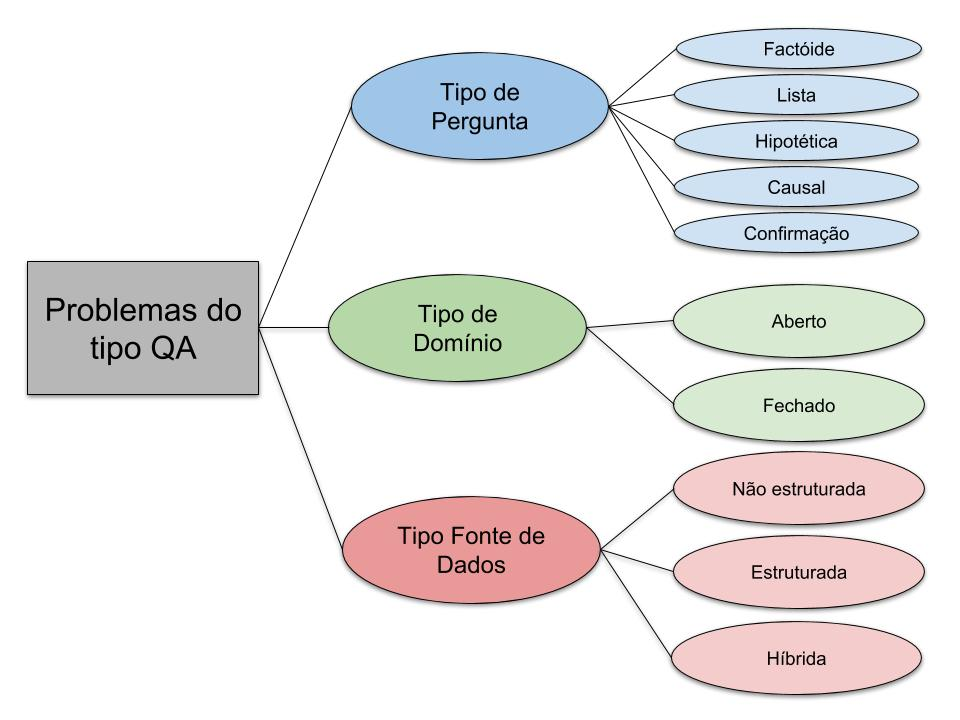
\includegraphics[scale=0.3]{SistemaQA2.jpg}
\caption{Características de problemas do tipo QA [REDESENHAR. FIGURA FEIA.]}
\label{fig:SistemaQA}
\end{figure}

Os tipos das fontes de dados acessadas têm forte influência sobre as arquiteturas que serão utilizadas na implementação dos sistemas que se propõem tratar problemas do tipo QA. De acordo com \citep{speech}, existem 3 principais paradigmas para tratar problemas do tipo QA: "Information Retrieval" (IR), "Knowledge Based" (KB) MORREU e PRECISO ENCAIXAR[ou NLIDB], e Híbridas (HIB), respectivamente para tipos de fontes de dados não estruturadas, estruturadas e estruturadas + não estruturadas.\\

O paradigma Information Retrieval (IR) ...\\

São chamados de "Sistemas Question Answering Information Retrieval" (Sistemas QA-IR) os sistemas que se propõem tratar problemas do tipo QA e utilizam o paradigma IR para responder perguntas escritas em linguagem natural a partir de fontes de dados não estruturadas.\\

Apresentar os principais componentes da arquitetura de Sistemas IR \citep{kolomiyets2011survey}. ACHEI ESSE ARTIGO QUE É DE 2017 E DE UM PERIÓDICO A1 (KNOWLEDGE-BASED SYSTEMS) COM APENAS 2 REFERÊNCIAS: A study about the future evaluation of Question-Answering systems (In this paper, we overview the main QA evaluations over free text, paying special attention to the changes encouraged at such campaigns). DAR UMA LIDA NELE!\\

O paradigma Knowledge Based (KB) ...\\

São chamados de "Sistemas Question Answering Knowledge Based" (Sistemas QA-KB) os sistemas que se propõem tratar problemas do tipo QA e utilizam o paradigma KB para responder perguntas escritas em linguagem natural a partir de fontes de dados estruturadas. FALAR DA CONVERSÃO PARA FORMA LÓGICA\\

Apresentar os principais componentes da arquitetura de Sistemas KB\\

Uma especialização dos sistemas QA-KB são os sistemas Natural Language Interface to Database (NLIDB) que respondem perguntas escritas em linguagem natural a partir de bases de dados estruturadas relacionais [REF]. O estudo dos sistemas NLIDB é o foco desse trabalho.\\

O paradigma Híbrido (HIB) ...\\

São chamados de "Sistemas Question Answering Híbridos" (Sistemas QA-HIB) os sistemas que se propõem tratar problemas do tipo QA e utilizam o paradigma HIB para responder perguntas escritas em linguagem natural a partir de fontes de dados estruturadas e não estruturadas.\\

Apresentar os principais componentes da arquitetura de Sistemas Híbridos.\\

A figura \ref{fig:TiposDeSistemasQA} apresenta uma visão consolidada dos diferentes tipos de sistemas QA discutidos até agora.\\

\begin{figure}[h!]
\centering
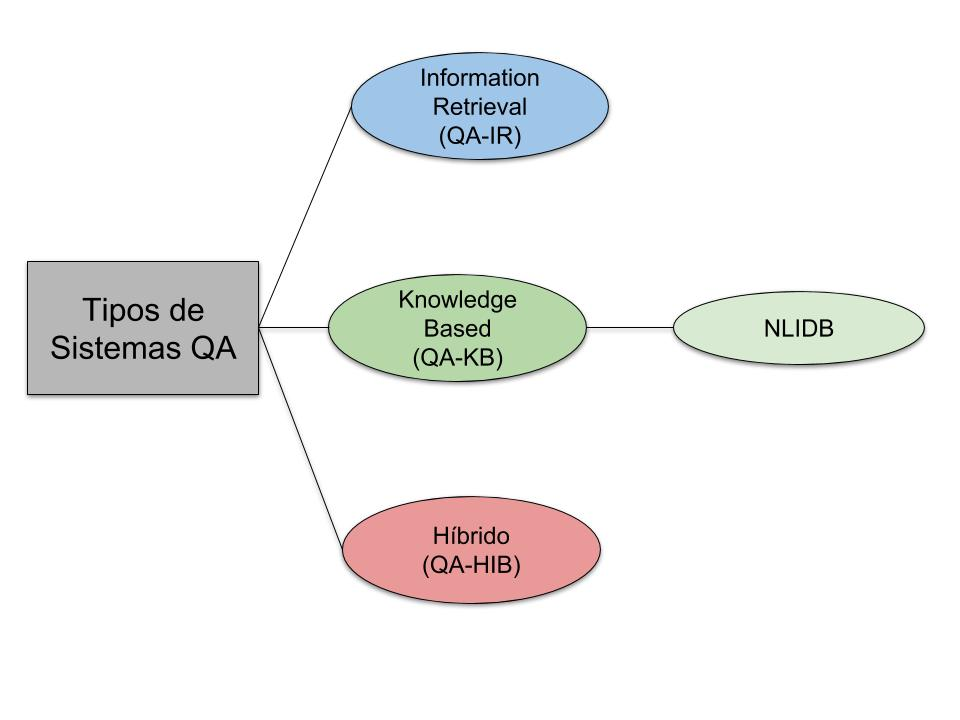
\includegraphics[scale=0.3]{TiposDeSistemasQA.jpg}
\caption{Tipos de sistemas QA [REDESENHAR. FIGURA FEIA.]}
\label{fig:TiposDeSistemasQA}
\end{figure}

O objetivo desse trabalho é fazer um levantamento dos sistemas NLIDB. A seção \ref{sistemasKB} falará sobre os diferentes tipos de PROBLEMA (TROCAR EM TODAS AS PARTES DO TEXTO) QA KB. A seção \ref{exemplosSistemasKB} falará sobre exemplos de sistemas QA KB. Por fim, a seção \ref{conclusoes} apresenta as conclusões.

%O objetivo desse trabalho é fazer um levantamento dos sistemas de QA que acessam bases de dados estruturadas (Sistemas KB ou NLIDB) para responder as perguntas do tipo factóide informadas pelos usuários em linguagem natural, independente do tipo de domínio (aberto ou fechado). A seção \ref{sistemasKB} falará sobre os diferentes tipos de PROBLEMA (TROCAR EM TODAS AS PARTES DO TEXTO) QA KB. A seção \ref{exemplosSistemasKB} falará sobre exemplos de sistemas QA KB. Por fim, a seção \ref{conclusoes} apresenta as conclusões.


%É possível descrever sistemas QA que respondem factóides a partir de suas características, por exemplo, domínio da pergunta e tipo de fonte de dados.\\

%São exemplos de características de sistemas QA: domínio e tipo das perguntas suportadas \citep{mishra2016survey}. [Checar essas referências também \citep{lopez2011question} e \citep{hirschman2001natural} para a definição de um sistema QA]\\



%Os tipos de perguntas podem ser factóide, lista, hipotética, causal e confirmação. O tipo factóide .... O tipo lista .... O tipo hipotética .... O tipo causal .... Por fim, o tipo confirmação .... Para o restante desse trabalho, os tipos de pergunta factóide e lista serão tratados como um único tipo e serão chamados de factóide.\\

%Independente da característica "domínio da pergunta", sistemas QA que suportam "tipo de pergunta" factóide são tipicamente resolvidos por modelos IR, KB ou Híbridos. Modelos IR são utilizados quando a fonte de dados acessada pelo sistema QA são não-estruturadas. Caso a fonte de dados do sistema QA seja estruturada, modelos KB são utilizados. Por fim, caso a fonte de dados seja composta por dados não-estruturados e estruturados, modelos híbridos são adotados \citep{livroStanford}.\\



%Modelos IR são utilizados quando a fonte de dados acessada pelo sistema QA são não-estruturadas. Caso a fonte de dados do sistema QA seja estruturada, modelos KB são utilizados. Por fim, caso a fonte de dados seja composta por dados não-estruturados e estruturados, modelos híbridos são adotados \citep{livroStanford}.\\

%Para os sistemas que suportam perguntas do tipo factóide, caso os dados sejam não estruturados, sistemas de QA são chamados de Information Retrieval. Caso os dados sejam estruturados, sistemas de QA são chamados de Knowledge Based .  Sistemas que trabalham com as duas abordagens são conhecidos como Híbridos\\

%Sistemas Information Retrieval (IR) são...\\

%Sistemas Knowledge Based (KB) são .... Sistemas KB também são conhecidos como Natural Language Interfaces to Databases \citep{androutsopoulos1995natural}. \\

%Sistemas Híbridos...\\



%===========================================================
%===========================================================
%===========================================================
%===========================================================

\section{Acho que preciso de uma seção sobre metodologia\label{metodologia}}

%\section{Sistemas Question Answering Knowledge Based (QA-KB)\label{sistemasKB}}

\section{Sistemas Natural Language Interface to Databases (NLIDB)\label{sistemasNLIDB}}

O trabalho \citep{androutsopoulos1995natural} é uma introdução para o problema \textit{Natural Language Interface to DataBases} (NLIDB). Ele apresenta algumas vantagens e desvantagens dos modelos NLIDB quando comparados com linguagens formais de consultas a bancos de dados, por exemplo, SQL, interfaces baseadas em formulários e interfaces gráficas. Ele também discute questões arquiteturais e de portabilidade. \\

Sistemas NLIDB recebem consultas em linguagem natural e retornam resultados a partir de fontes de dados estruturadas relacionais. Implementações desse tipo de sistemas podem ser classificadas como: baseado em gramática, baseado em regras, baseado em síntese de programas e baseado em redes neurais\citep{speech}.\\

[Existe algo para mais de uma tabela? Pode ser um diferencial! Talvez possa falar aqui que uma limitação é que todas as abordagens utilizam uma única tabela.]\\

[LER ESSE ARTIGO
Knowledge-based question answering using the semantic embedding space https://www.sciencedirect.com/science/article/pii/S0957417415004698]


A figura \ref{fig:SistemaNLIDB} apresenta tipos de implementações/soluções de sistemas NLIDB discutidas anteriormente.

%exemplo de figura
\begin{figure}[h!]
\centering
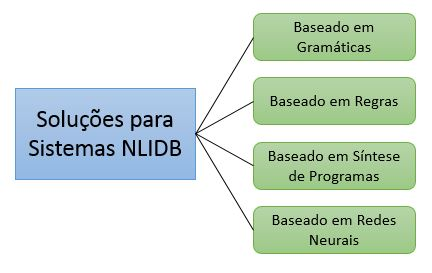
\includegraphics[scale=0.7]{NLIDB.JPG}
\caption{Tipos de implementações/soluções de sistemas NLIDB [REDESENHAR. FIGURA FEIA.]}
\label{fig:SistemaNLIDB}
\end{figure}

\subsection{Sistemas NLIDB baseados em gramáticas}

Explicar o que são sistemas NLIDB baseados em gramáticas.

\subsection{Sistemas NLIDB baseados em regras}

Explicar o que são sistemas NLIDB baseados em regras\\

\subsection{Sistemas NLIDB baseados em Síntese de Programas}

Explicar o que são sistemas NLIDB baseados em Síntese de Programas\\

\subsection{Sistemas NLIDB baseados em Redes Neurais}

Explicar o que são sistemas NLIDB baseados em Redes Neurais\\


TODO0: PEGAR ARTIGOS DO GIT

TODO1: Escrever o que li sobre síntese de programas para criar um ou dois parágrafos.

\citep{gulwani2017program}
\citep{yaghmazadeh2017sqlizer}

https://alexpolozov.com/blog/program-synthesis-2018/
Survey de síntese de programas: https://www.microsoft.com/en-us/research/wp-content/uploads/2017/10/program_synthesis_now.pdf

https://homes.cs.washington.edu/~bornholt/post/synthesis-explained.html








Falar das soluções baseadas em redes neurais (também chamados de NL2SQL e Text-to-SQL) [ACREDITO QUE NÃO PRECISA CRIAR UMA SUBSEÇÃO PARA ISSO].\\

[Olhar blog de síntese de programas da Aline. quais as relações com as redes neurais? Existe SP co ML e sem ML.]. 1 - program synthesis: https://alexpolozov.com/blog/program-synthesis-2018/ ele fala do survey que eu mencionei, e ele menciona o dataset WikiSQL, na parte de datasets.



%===========================================================
%===========================================================
%===========================================================
%===========================================================

\section{Levantamento de Sistemas NLIDB\label{exemplosSistemasNLIDB}}

A seção \ref{sistemasNLIDB} apresentou os tipos de sistemas NLIDB, que são baseados em gramáticas, regras, síntese de programas e redes neurais. O objetivo dessa seção é apresentar exemplos de sistemas NLIDB.\\

As seções \ref{velhos} e \ref{novos} apresentarão com detalhes os sistemas descritos na tabela abaixo \ref{table:exemplos}.

%https://www.tablesgenerator.com/
\begin{table}[]
\centering
\begin{tabular}{|c|c|c|c|c|}
\hline
a & a & a & a & a \\ \hline
b & b & b & b & b \\ \hline
c & c & c & c & c \\ \hline
d & d & d & d & d \\ \hline
\end{tabular}
\caption{Tabela comparativa das soluções NLIDB}
\label{table:exemplos}
\end{table}

\subsection{Trabalhos NLIDB antigos\label{velhos}}

Protótipos de sistemas NLIDB apareceram no final dos anos 60. Nessa época, o NLIDB mais conhecido era LUNAR \citep{woods1973progress}, uma interface em linguagem natural para um banco de dados de análises químicas de rochas lunares. Esse sistema é concentrado em um domínio de informação. Era baseado em regras, sup ou semi-sup?\\

RENDEZVOUS \citep{codd1974seven} engajava os usuários em diálogos para ajudá-los a formular suas consultas. Domínio aberto ou fechado? Era baseado em regras, sup ou semi-sup?\\

LADDER \citep{hendrix1978developing} usava gramáticas semânticas, uma técnica que intercala processamento sintático e semântico. Essa estratégia gerava dificuldades para o uso do sistema em outros domínios uma vez que demandava a criação de uma outra gramática. Era baseado em regras, sup ou semi-sup?\\

Conforme pesquisadores passaram a concentrar esforços em sistemas de domínio aberto, sistemas baseados em "semantic grammars" passaram a ser abandonados. PLANES \citep{waltz1978english} e PHILIQA1 \citep{scha1977philips} foram outros sistemas que apareceram no final dos anos 70. Eram de domínio aberto ou fechado? Eram baseados em regras, sup ou semi-sup?\\

CHAT80 \citep{warren1982efficient} é um dos sistemas mais conhecidos do início dos anos 80. Foi implementado em PROLOG e transformava consultas escritas em inglês para expressões PROLOG, que eram avaliadas em bancos de dados PROLOG. Eram de domínio aberto ou fechado? Eram baseados em regras, sup ou semi-sup?\\

No meio dos anos 80, NLIDBs eram uma área muito popular de pesquisa. Grande parte dos pesquisadores se interessavam por questões do portabilidade, ou seja, sistemas aplicáveis a diferentes domínios. Por exemplo, o sistema TEAM \citep{grosz1983team} foi projetado para ser facilmente configurável sem conhecimento do banco de dados utilizado. Era baseado em regras, sup ou semi-sup?\\

ASK \citep{thompson1983introducing} permitia que usuários finais ensinassem ao sistema novas palavras e conceitos em qualquer momento da interação. Ele tinha um sistema gerenciador de banco de dados interno e tinha a habilidade de interagir com outras bases externas, programas de email eletrônico e outras aplicações. Era de domínio aberto ou fechado? Era baseado em regras, sup ou semi-sup?\\

JANUS \citep{hinrichs1988tense} tinha a mesma habilidade de conectar a outras sistemas (bancos de dados, sistemas especialistas, dispositivos gráficos, etc). Dessa forma, ele abstraia a complexidade dos sistemas provedores de informação para o usuário final. Além disso, ele era um dos poucos a suportar questões temporais. Era de domínio aberto ou fechado? Era baseado em regras, sup ou semi-sup?\\

Diversos outros sistemas apareceram nos anos 80, por exemplo DATALOG \citep{hafner1984interaction}, EUFID \citep{templeton1983problems}, LDC \citep{ballard1984ldc}, TQA \citep{damerau1981operating} e TELI \citep{ballard1986semantic}. Eram de domínio aberto ou fechado? Eram baseados em regras, sup ou semi-sup?\\

De acordo com \citep{johnson1984natural} em 1987, tecnologias NLIDB seriam o padrão para usuários de DBMSs e haveria um conjunto de alternativas de produtos. Entretanto, essa previsão não se confirmou por alguns motivos: evolução das interfaces gráficas, ...\\

Outros trabalhos mais recentes...\\

A dissertação de mestrado \citep{chandra2006natural} propõe um modelo baseado em grafos. O sistema faz a coleta de todas as informações possíveis de bancos de dados e sentenças existentes, e transforma essas informações em uma base de conhecimento para o sistema. Dado uma nova pergunta, o sistema irá usar o conhecimento para analisar e traduzir a sentença em uma \textit{query} correspondente. \\

O trabalho \cite{popescu2003towards} introduz a definição de "perguntas semanticamente tratáveis" e a implementação de um modelo chamado "PRECISE NLI". O modelo PRECISE funcionou muito bem com bases de testes de perguntas "semanticamente tratáveis". O problema é que esse tipo de pergunta exige que as perguntas sejam escritas respeitando um conjunto de regras, por exemplo, que um atributo venha sempre precedido de palavras como \textit{"What"} e \textit{"Who"}. Essa é uma grande limitação do modelo. \\

O trabalho \citep{minock2005phrasal} apresenta o modelo STED que tem a habilidade de entender e gerar frases em linguagem natural para engajar o usuário na clarificação dos diálogos quando há dúvidas na pergunta de entrada. \\

Conforme o trabalho \citep{akula2013novel}, usuários falham em expressas suas intenções em apenas uma pergunta em linguagem natural. Assim, para responder uma sequência de perguntas em linguagem natural, sistemas NLIDB precisam capturar e manter o contexto do usuário. \\

O trabalho \citep{li2014constructing} propõe o modelo NaLIR \\

A Microsoft já teve seu produto NLIDB, chamado "Microsoft English Query", mas ele foi descontinuado em 2008 (https://www.infoq.com/news/English-Query-Discontinued).\\

\subsection{Trabalhos NLIDB NOVOS\label{novos}}

Mais recentemente novos modelos supervisionados baseados em Síntese de Programas e em Redes Neurais vem sendo propostos. Esses modelos serão detalhados a seguir.\\

Uma abordagem muito usada são Modelos KB SUP baseados em síntese de programas.\\

O trabalho \citep{yaghmazadeh2017sqlizer} propõe o SQLizer que é um modelo baseado em síntese de programas. \\

O trabalho \citep{zelle1996learning} apresenta o CHILL que usa técnicas de Programação Lógica Indutiva para gerar consultas na forma lógica.

Recentemente houve um crescimento de modelos KB SUP baseados em redes neurais.\\

O trabalho \citep{zhong2017seq2sql} apresentou um \textit{dataset} de 80654 perguntas anotadas manualmente para apoiar processos de treinamento de modelos NLIDB chamado WikiSQL. Além disso, ele também propôs o modelo Seq2SQL, uma rede neural profunda para tradução de perguntas em linguagem natural para consultas SQL. \\

Após a criação do WikiSQL, diversos trabalhos foram publicados. Seguem esses trabalhos em ordem de publicação. Essa ordem também respeita a posição no ranking (https://github.com/salesforce/WikiSQL) da última para a primeira posição.\\

O trabalho \citep{wang2018pointing} usa um modelo \textit{sequence to sequence} onde o \textit{decoder} usa um modelo simples de digitação de expressões SQL para estruturar a predição da saída. \\

O trabalho \citep{xu2017sqlnet} utiliza uma estratégia baseada em \textit{sketchs} que armazena um grafo de dependências de tal forma que uma predição pode ser feita considerando apenas as predições anteriores que ele depende. \\

O trabalho \citep{huang2018natural} explora um protocolo diferente de aprendizado ... \\

O trabalho \citep{yu2018typesql} apresenta a estratégia TypeSQL, que vê problemas NLIDB como uma tarefa "\textit{slot filling}". Eles também mostram que acessando o conteúdo de bancos de dados pode melhorar significativamente os resultados quando as perguntas dos usuários não são bem formadas. \\

O trabalho \citep{dong2018coarse} decompõe o processo de \textit{parsing} semântico em 2 etapas. Primeiro ele gera um \textit{sketch} da consulta SQL e depois preenche as lacunas da \textit{sketch}. \\

O trabalho \cite{mccann2018natural} introduz o desafio "\textit{Natural Language Decathlon}" (decaNLP), que possui 10 tipos de tarefas: question answering, machine translation, summarization, natural language inference, sentiment analysis, semantic role labeling, zero-shot relation extraction, goal-oriented dialogue, semantic parsing, and commonsense pronoun resolution. Além disso, eles apresentam uma rede multitarefa chamada "\textit{Multitask Question Answering Network}" (MQAN) que é capaz de aprender todas as tarefas do decaNLP sem módulos, parâmetros ou configurações específicos. \\

O trabalho \citep{2018arXiv180703100W} detecta e exclui programas falhos durante o processo de decodificação através da execução do programa parcialmente gerado. \\

O trabalho \citep{shi2018incsql} atualmente é o primeiro do ranking WikiSQL (18/09/2018). Ele ainda é um relatório técnico em elaboração. Ele citou o trabalho \citep{finegan2018improving} (ACL 2018) que propõe uma metodologia de avaliação para problemas chamados de \textit{Text-to-SQL}.\\

%===========================================================
%===========================================================
%===========================================================
%===========================================================

\section{Conclusões\label{conclusoes}}

PROBLEMAS EM ABERTO\\

TENDÊNCIAS\\

Criar modelo para considerar mais de uma tabela?\\

Geração de linguagem intermediária? 2 - Universal Language Model, que foi publicado no ACL 2018: http://nlp.fast.ai/classification/2018/05/15/introducting-ulmfit.html.\\

3 - Vários problemas de NLP resolvidos com a mesma topologia de rede (baseada em atenção) do OpenAI: https://blog.openai.com/language-unsupervised/\\

%===========================================================
%===========================================================
%===========================================================
%===========================================================






%exemplo de figura
%\begin{figure}[h!]
%\centering
%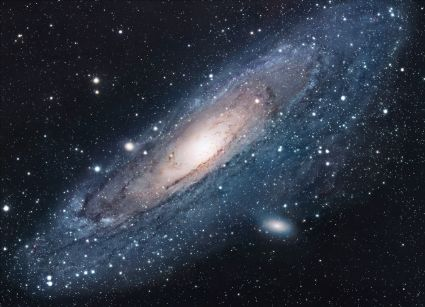
\includegraphics[scale=1.7]{universe}
%\caption{The Universe}
%\label{fig:universe}
%\end{figure}

%======================================================================================
%======================================================================================
%======================================================================================
%\section{Old}

%[DÚVIDA: VOU FAZER ESSA SEÇÃO EM LINHA DO TEMPO OU AGRUPANDO PELOS TIPOS?]\\

%Falar sobre os exemplos dos anos 70 e 80 e em quais tipos eles se encaixam: regras, superv ou semi-superv. Também é importante destacar os datasets utilizados...\\

%Mais recentemente, estratégias supervisionadas baseadas em INDUÇÃO DE PROGRAMAS\\

%Outros trabalhos vem sendo feitos através de redes neurais.\\

%O trabalho \citep{zhong2017seq2sql} propôs a criação do \textit{dataset} WikiSQL, conjunto de pares de perguntas em linguagens natural e queries SQL. Diversos trabalhos propuseram soluções testadas sobre esse \textit{dataset}.\\

%Falar sobre todos os trabalhos do WikiSQL. Para cada uma das soluções é importante falar do tipo: regras, superv ou semi-super\\

%======================================================================================
%======================================================================================
%======================================================================================

%\section{Qual o objetivo da tese?}

%Qual o objetivo do trabalho?\\

%Esse trabalho propõe o CCRNet, que é um modelo de conversão de consultas a bancos de dados relacionais escritas em linguagem natural para queries SQL, independente do modelo de dados utilizado, ou seja, capaz de ser utilizado para a realização de consultas em modelos de dados de diferentes áreas de conhecimento (database agnostic). Além disso, para o idioma português é proposto um plugin (CCRNetBR) que tem como objetivo otimizar os resultados para o idioma específico.\\

%Tirar a palavra "modelo" de dados do objetivo. Trocar por schema (schema agnostic).\\

%Esse modelo será avaliado pelos resultados obtidos nas suas execuções frente a diferentes datasets (https://atlas.cern/tags/open-data, WikiSQL - MAS, IMDB e YELP).\\

%Como os outros modelos funcionam? O que proporei de diferente para o meu modelo?\\

%Para responder essa pergunta preciso verificar os tipos de solução. Acredito que os surveys apresentam arquiteturas com os tipos de soluções. Preciso descobrir em qual tipo de solução os modelos NL2SQL se encaixam. Dessa forma, consigo encaixar os artigos antigos com os artigos atuais que tratam o WikiSQL.\\

%Também é importante encaixar o modelo síntese automática de queries SQL.\\

%AGORA já! Pensar em ideias antes de aprofundar o conhecimento.\\

%Aprofundar estudo em uma solução NL2SQL e ver como funciona a rede LSTM nesse caso. Preciso conseguir explicar com detalhes como funciona um exemplo do wikisql. Como a saída SQL é avaliada no wikiSQL para ganhar uma nota?\\

%\section{Sobre os Datasets}

%\section{Pesquisa Bibliográfica}


%ACHO QUE VOU REMOVER O trabalho \citep{kolomiyets2011survey} também é uma introdução. Ele explica as diferenças entre "\textit{Question Answering}" e "\textit{Information Retrieveal}" e NLIDBs. Segundo ele, NLIDB é a origem de QA, mas QA expandiu a ideia de pesquisa para outras fontes de dados diferentes de bancos relacionais. \\

%ACHO QUE VOU REMOVER O trabalho \citep{pazos2013natural} apresenta um estudo sobre sistemas NLIDB. Ele discute questões como classificação, técnicas, vantagens, desvantagens, e uma proposta para uma avaliação apropriada deles. \\

%ACHO QUE VOU REMOVER O trabalho \citep{mishra2016survey} faz um resumo sobre trabalhos QA e os classifica com base em diferentes critérios, como: domínio da aplicação, tipos de pergunta (what, when, which, who e how), tipo da análise da pergunta (semântica, sintática, morfológica), fontes de dados (estruturados, semi-estruturados e não estruturados). \\




%======================================================================================



%======================================================================================



%======================================================================================

\bibliographystyle{plain}
\bibliography{references}
\end{document}